% Regression slice derived from the PGF shapes.multipart manual.
% A record box can opt into per-part fill and explicitly return to its normal
% node background with `rectangle split uses custom fill=false`.
\documentclass[tikz,border=2pt]{standalone}
\usetikzlibrary{shapes.multipart}
\begin{document}
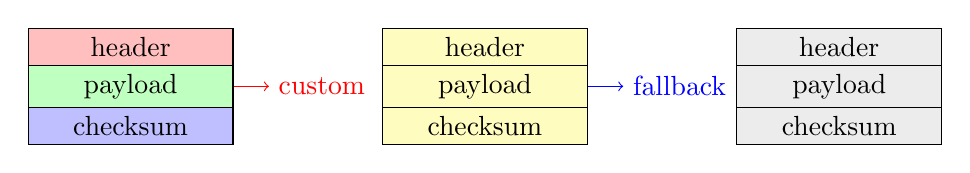
\begin{tikzpicture}[
  record/.style={
    rectangle split,
    rectangle split parts=3,
    draw,
    minimum width=2.6cm,
    inner sep=3pt
  }
]
  \node[record, rectangle split part fill={red!25,green!25,blue!25}] (custom) at (0,0)
    {header\nodepart{two}payload\nodepart{three}checksum};
  \node[record, rectangle split part fill={red!25,green!25,blue!25},
    rectangle split uses custom fill=false, fill=yellow!25] (fallback) at (4.5,0)
    {header\nodepart{two}payload\nodepart{three}checksum};
  \node[record, fill=gray!15] (plain) at (9,0)
    {header\nodepart{two}payload\nodepart{three}checksum};

  \draw[->,red] (custom.two east) -- ++(.45,0) node[right] {custom};
  \draw[->,blue] (fallback.two east) -- ++(.45,0) node[right] {fallback};
\end{tikzpicture}
\end{document}
